\chapter{Wie erstelle ich einen Kellerautomaten?}\label{PDA}


Wie ein normaler Automat angelegt wird, wurde bereits besprochen. In diesem
Kapitel geht es darum einen Kellerautomaten anzulegen der die Sprache $a^n b^n$
für $n \geq 0$ erkennt. Als erstes muss der Neu-Dialog geöffnet werden, im ersten
Tab muss der "`Automat"' gewählt werden, anschließend der "`Kellerautomat"'. Für
das Beispiel muss sowohl als Eingabe- wie auch als Kelleralphabet das Alphabet
\{\Symbol{a}, \Symbol{b}\} gewählt werden. Dazu kann das Alphabet bei beiden
Eingabefeldern einzeln eingestellt werden, oder nur bei "`Eingabe Alphabet"',
wobei dann der Haken bei "`Keller Alphabet"' entfernt werden muss. Dadurch werden
automatisch die gleichen Alphabete verwendet.\vspace{10pt}

Ist die Datei angelegt, muss überlegt werden, welche Zustände und Übergänge
benötigt werden, um die Sprache zu erkennen. Dabei kommt man dazu, dass
mindestens folgende Zustände und Übergänge nötig sind, um die Sprache zu
erkennen:

\begin{itemize}
  \item Ein Zustand \State{z0} der sowohl Start, wie auch akzeptierenden
  Zustand ist
  \item Ein Zustand \State{z1}
  \item Ein akzeptierender Zustand \State{z2}
  \item Einen Übergang von \State{z0} nach \State{z1} der das erste Symbol
  \Symbol{a} vom Eingabewort liest und auf den Keller schreibt
  \item Einen Übergang von \State{z1} nach \State{z1} der alle weiteren Symbole
  \Symbol{a} vom Eingabewort liest und auf den Keller schreibt
  \item Einen Übergang von \State{z1} nach \State{z2} der das erste \Symbol{b}
  vom Eingabeband liest und das oberste \Symbol{a} vom Keller löscht.
  \item Einen Übergang von \State{z2} nach \State{z2} der alle weiteren
  Symbole \Symbol{b} vom Eingabewort liest und die entsprechenden Symbole
  \Symbol{a} vom Keller löscht
\end{itemize}

\begin{figure}[h]
\begin{center}
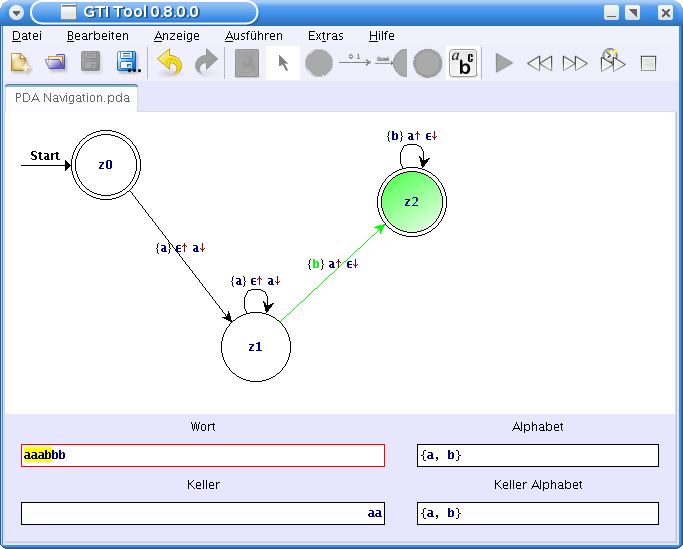
\includegraphics[width=12cm]{images/pda_navigation.png}
\caption{Kellerautomat Navigation}
\end{center}
\end{figure}

Bei der Wort Navigation muss sich somit ergeben, damit das Wort akzeptiert wird,
dass das Eingabewort komplett gelesen wurde und sich der Automat entweder im
Zustand \State{z0} befindet, was bedeutet, dass das Eingabewort leer war, oder,
dass sich der Automat im Zustand \State{z2} befindet und der Keller leer
ist.\vspace{10pt}

Wie die Zustände und Übergänge angelegt werden, wurde bereits in diesem Handbuch
beschrieben, deshalb wird an dieser Stelle nur auf die Besonderheiten des
Kellerautomaten eingegangen. Es werden insgesamt vier Übergänge benötigt, um die
Sprache zu erkennen. Alle Übergänge müssen Veränderungen am Keller durchführen.
Wir nehmen als Beispiel den Übergang von \State{z0} nach \State{z1}, bei dem das
Symbol \Symbol{a} vom Eingabeband gelesen und auf den Keller geschrieben werden
muss. Beim Anlegen oder Editeren dieser Transition besteht die Möglichkeit das
"`Keller Lese-Wort"' und das "`Keller Schreib-Wort"' zu editieren. In diesem Fall
soll das Symbol \Symbol{a} auf den Keller geschrieben werden, es muss also beim
"`Keller Schreib-Wort"' das Symbol \Symbol{a} eingetragen werden. Das "`Keller
Lese-Wort"' muss leer bleiben, da nichts vom Keller gelesen werden
soll.\vspace{10pt}


\section{Navigation}

Wurden auf diese Weise alle Zustände und Übergange angelegt, kann der Automat
validiert werden und sollte keine Fehler mehr aufweisen. Bei der Wort
Navigation ist jetzt nicht nur das Eingabewort interessant, sondern auch der
dargestellte Keller. Wird zum Beispiel das Wort \Word{aaabbb} gewählt, wird im
ersten Schritt das Symbol \Symbol{a} gelesen und auf den Keller geschrieben.
Anschließend werden die restlichen zwei Symbole \Symbol{a} auf den Keller
gepackt und anschließend durch die Übergänge von \State{z1} nach \State{z2}
bzw. von \State{z2} nach \State{z2} wieder entfernt. Am Ende wurde das
komplette Wort \Word{aaabbb} gelesen, der Automat befindet sich im Zustand
\State{z2} und der Keller ist leer, das Wort wird somit akzeptiert.


\section{Kellerautomat aus Grammatik erstellen}

Im folgenden soll ein Sonderfall der Navigation mit dem Kellerautomat betrachtet
werden. Dazu muss die Grammatik erstellt werden, die Wörter der Form $a^n b^n$
für $n \geq 0$ erkennt. Wie in Kapitel \ref{Grammar} angegeben, müssen die beiden
Produktionen \StartSymbol{E} $\to$ \TerminalSymbol{$\epsilon$} und
\StartSymbol{E} $\to$ \TerminalSymbol{a}\StartSymbol{E}\TerminalSymbol{b}
angelegt werden. Anschließend wandeln wir die Grammatik in einen
Kellerautomaten um, dies erfolgt mit "`Umwandel in\ldots"' im Menüpunkt
"`Ausführen"'. Bei dieser Art der Umwandlung entsteht immer ein Kellerautomat
mit zwei Zuständen \State{s} und \State{f}. Der Unterschied zu normalen
Automaten ist, dass jetzt vom Zustand \State{f} mehrere Übergänge in sich
selbst existieren, so dass eine Beschriftung des Überganges keinen Sinn hätte.
Welche Übergänge genau vorhanden sind, kann in der "`Keller Operationen"'
Tabelle nachgesehen werden.\vspace{10pt}

\begin{figure}[h]
\begin{center}
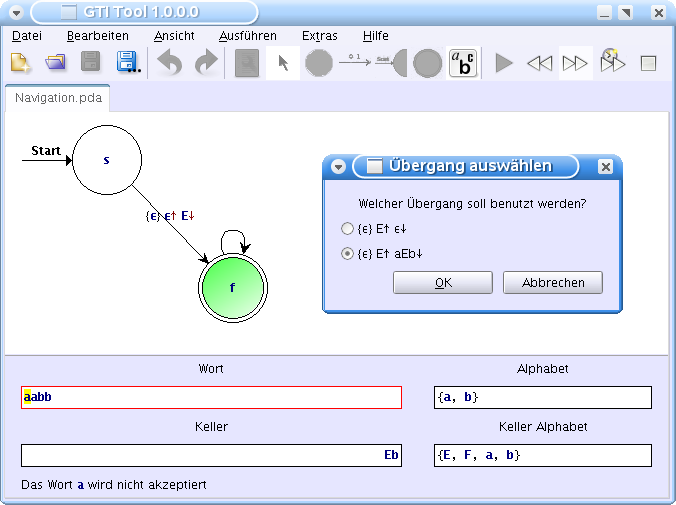
\includegraphics[width=12cm]{images/grammar_pda.png}
\caption{Grammatik - Kellerautomat Navigation}
\end{center}
\end{figure}

Wird für diesen Automaten die Wordnavigation mit dem Wort \Word{aabb} gestartet,
ergibt sich im zweiten Schritt der Navigation, dass der Übergang der verwendet
werden kann, nicht mehr eindeutig ist. Oben auf dem Keller befindet sich das
Nichtterminalzeichen \StartSymbol{E}, welches entweder durch
\TerminalSymbol{$\epsilon$} oder durch
\TerminalSymbol{a}\StartSymbol{E}\TerminalSymbol{b} ersetzt werden könnte. Da
wir das Wort \Word{aabb} erkennen wollen, muss der Übergang \StartSymbol{E}
$\to$ \TerminalSymbol{a}\StartSymbol{E}\TerminalSymbol{b} ausgewählt werden.
Der nächste Schritt ist wieder eindeutig, da nur der Übergang ausgewählt werden
kann, der \TerminalSymbol{a} vom Eingabewort liest und \TerminalSymbol{a} vom
Keller entfernt. Im nächsten Schritt muss wieder ausgewählt werden, welcher
Übergang verwendet werden soll. Da als nächstes Terminalzeichen wieder ein
\TerminalSymbol{a} auf dem Eingabewort steht, muss wieder der Übergang \StartSymbol{E}
$\to$ \TerminalSymbol{a}\StartSymbol{E}\TerminalSymbol{b} ausgewählt werden.
Genau wie zuvor ist der nächste Schritt wieder eindeuting. Da als nächstes das
Terminalzeichen \TerminalSymbol{b} auf dem Keller steht, muss diesmal der
Übergang \StartSymbol{E} $\to$ \TerminalSymbol{$\epsilon$} ausgewählt werden.
Durch diesen Übergang wird das oben auf dem Keller stehende
Nichtterminalzeichen \StartSymbol{E} entfernt. Mit den nächsten zwei
eindeutigen Schritten werden die Terminalzeichen \TerminalSymbol{b} auf dem
Eingabewort gelesen und vom Keller entfernt. Da am Ende der Keller leer ist und
der Zustand \State{f} aktiv ist, wird das Wort akzeptiert.